% TikZ overview plot for operational metrics
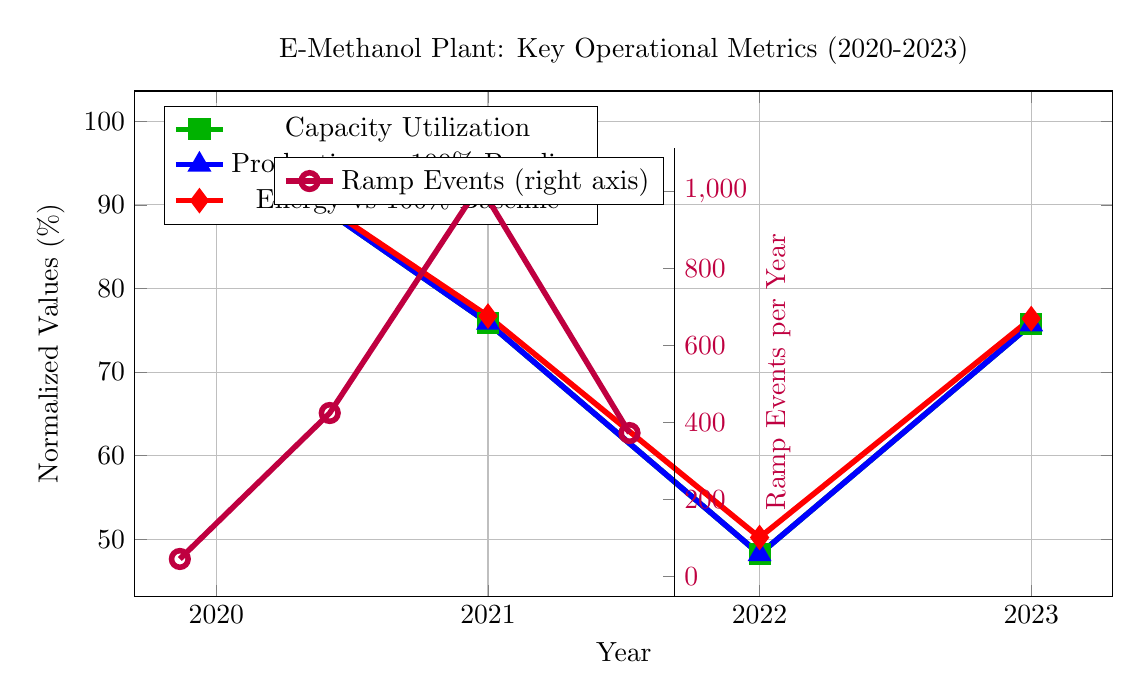
\begin{tikzpicture}
\begin{axis}[
    title={E-Methanol Plant: Key Operational Metrics (2020-2023)},
    xlabel={Year},
    ylabel={Normalized Values (\%)},
    width=14cm,
    height=8cm,
    xtick=data,
    xticklabels={2020, 2021, 2022, 2023},
    grid=major,
    legend pos=north west,
    mark options={solid},
]

\addplot[color=green!70!black, mark=square*, mark size=3pt, line width=2pt] coordinates {
    (2020, 98.5)
    (2021, 75.9)
    (2022, 48.2)
    (2023, 75.7)
};
\addlegendentry{Capacity Utilization}

\addplot[color=blue, mark=triangle*, mark size=3pt, line width=2pt] coordinates {
    (2020, 98.5)
    (2021, 75.9)
    (2022, 48.2)
    (2023, 75.7)
};
\addlegendentry{Production vs 100\% Baseline}

\addplot[color=red, mark=diamond*, mark size=3pt, line width=2pt] coordinates {
    (2020, 98.6)
    (2021, 76.7)
    (2022, 50.2)
    (2023, 76.4)
};
\addlegendentry{Energy vs 100\% Baseline}

\end{axis}

\begin{axis}[
    axis y line*=right,
    axis x line=none,
    ylabel near ticks,
    ylabel={Ramp Events per Year},
    yticklabel style={color=purple},
    ylabel style={color=purple},
    xtick=data,
    xticklabels={2020, 2021, 2022, 2023},
]

\addplot[color=purple, mark=o, mark size=3pt, line width=2pt] coordinates {
    (2020, 45)
    (2021, 424)
    (2022, 1015)
    (2023, 372)
};
\addlegendentry{Ramp Events (right axis)}

\end{axis}
\end{tikzpicture}
